\begin{center}
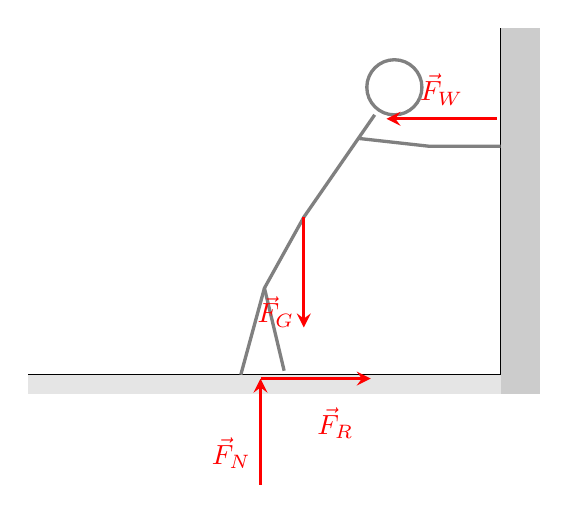
\begin{tikzpicture}[>=stealth]
 \draw (-1.5,0) -- (4.5,0);
 \fill[gray!20] (-1.5,0) rectangle (4.5,-0.25);
 \fill[gray!40] (4.5,-0.25) rectangle (5,4.4);
 \draw (4.5,0) -- (4.5,4.4);
 \draw[gray, very thick] (1.2,0) -- (1.5,1.1) -- (2.0,2.0) -- (2.9,3.3);
 \draw[gray, very thick] (1.5,1.1) -- (1.75,0.05);
 \draw[gray, very thick] (3.15,3.65) circle (0.35);
 \draw[gray, very thick] (2.7,3.0) -- (3.6,2.9) -- (4.5,2.9);
 \draw[->, very thick, red] (2.0,2.0) -- (2.0,0.6);
 \node[red, left] at (2.0,0.8) {$\vec F_\text{G}$};
 \draw[->, very thick, red] (1.45,-1.4) -- (1.45,-0.05);
 \node[red, left] at (1.45,-1.0) {$\vec F_\text{N}$};
 \draw[->, very thick, red] (1.45,-0.05) -- (2.85,-0.05);
 \node[red, below] at (2.4,-0.3) {$\vec F_\text{R}$};
 \draw[->, very thick, red] (4.45,3.25) -- (3.05,3.25);
 \node[red, above] at (3.75,3.3) {$\vec F_\text{W}$};
\end{tikzpicture}
\end{center}

Von aussen wirken auf Sie:
\begin{itemize}
\item die Gewichtskraft $\vec F_\text{G}$ (die Erde zieht Sie an). Reaktionspartner: Sie ziehen die Erde mit gleich grosser Kraft an.
\item die Normalkraft $\vec F_\text{N}$ des Bodens auf die Füsse, nach oben. Reaktionspartner: Ihre Füsse drücken auf den Boden.
\item die Kraft $\vec F_\text{W}$ der Wand auf Ihre Hände, horizontal von der Wand weg. Reaktionspartner: Ihre Hände drücken gegen die Wand.
\item die Haftreibungskraft $\vec F_\text{R}$ des Bodens auf die Füsse, horizontal zur Wand hin. Reaktionspartner: Ihre Füsse stossen den Boden von der Wand weg.
\end{itemize}
Da Sie in Ruhe bleiben, ist $F_\text{N} = F_\text{G}$ und $F_\text{R} = F_\text{W}$. Ohne Haftreibung (z.B. auf Glatteis) würden Sie von der Wand weggeschoben.
